\section{Zielsetzung}
In diesem Versuch soll die Wellenlänge eines Lasers und der Brechungsindex der Luft mit Hilfe eines Michelson Interferometers
ermittelt werden.

\section{Theorie}
\subsection{Interferenz}
Um das Michelson Interferometer erklären zu können, muss zunächst einmal der Begriff \textbf{Interferenz} näher erläutert werden.

Das Licht kann durch eine elektromagnetische Welle der Form

\begin{equation*}
  \vec{E} = \vec{E}_0 cos(kx - \omega t - \delta)
\end{equation*}

beschrieben werden, wobei $\vec{E}_0$ die elektrische Feldstärke, $k$ die Wellenzahl, $\omega$ die Kreisfrequenz und $\delta$ den
Phasenwinkel beschreibt. Wenn für das Licht die Maxwell Gleichungen und somit das Superpostionsprinzip gilt, kann die bei einer Überlagerung
entstehende Welle durch die Addition der Vektoren bestimmt werden.

\begin{equation*}
  \vec{E} = \vec{E}_1 + \vec{E}_2 + ...
\end{equation*}

Da sich die elektrische Feldstärke in dem Frequenzbereich nicht messen lässt, werden im folgenden nur die Intensitäten betrachtet.

\begin{equation*}
  I = const |\vec{E}|^2
\end{equation*}

Somit kann man die Intensität zweier überlagerten Wellen als

\begin{equation*}
  I = 2 const \vec{E}_0^2 (cos(\delta_2 - \delta_1) + 1)
\end{equation*}

darstellen, wobei $ 2 const \vec{E}_0^2 cos(\delta_2 - \delta_1) $ als Interferenzterm bekannt ist. Zu erkennen ist, dass der Interferenzterm
minimal wird, wenn $\delta_2 - \delta_1$ ein ungerades Vielfache von $\pi$ ist, somit ist die Intensität $ I=0$. Die Intensität wird maximal, wenn
$\delta_2 - \delta_1$ null oder ein gerades Vielfaches von $\pi$ ist. Für den Interferenzeffekt ist also wichtig, welche Phasenverschiebung die beiden
überlagerten Wellen zueinander haben.
Eine zusätzliche Vorraussetzung für Interferenz ist die Kohärenz der Lichtstrahlen, also dass $k$, $\omega$ und $\delta$ zeitlich konstant sind. Dies lässt
sich praktisch durch Licht aus einer einzigen Lichtquelle umsetzen.

\subsection{Michelson-Interferometer}
In Abbildung \ref{Abb:1} ist der schematische Aufbau eines Michelson-Interferomenters abgebildet.

\begin{figure}
  \centering
  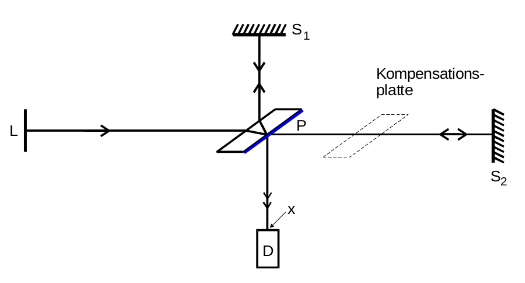
\includegraphics[scale = 0.5]{V401-Bild1.png}
  \caption{Schematischer Aufbaue eines Michelson-Interferometers \cite{Q1}.}
  \label{Abb:1}
\end{figure}

Hierbei ist L die Lichtquelle, $S_1$ und $S_2$ die Spiegel, $D$
der Detektor und P die semipermeable Platte. Das aus der Lichtquelle austretende Licht wird durch die semipermeable Platte in zwei Lichtstrahlen getrennt.
Der erste Lichtstrahl geht gerade durch die Platte und wird am Spiegel $S_2$ reflektiert, um sodann, von der Platte  abgelenkt, zum Detektor zu gelangen. Der andere Lichtstrahl
wird direkt von der Platte reflektiert und gelangt somit zum Spiegel $S_1$. Dort wird dieser reflektiert und gelangt, unreflektiert von der Platte, zum Detektor. Um die
Kohärenz der Strahlen beizubehalten, durchläuft der zweite Strahl eine Kompensationsplatte, außerdem müssen die Wege $\overline{PS_1}$ und $\overline{PS_1}$ nahezu identisch sein.
Das gewünschte Interferenzmuster entsteht durch einen Gangunterschied $w$  der beiden Strahlen, welcher sich durch das Verschieben des Spiegels um das Stück $d$ verändern lässt.

\begin{equation}
  w = 2d
\end{equation}

Ein Interferenzminimum entsteht bei einem Gangunterschied von

\begin{equation*}
  w = n \cdot \lambda, \; n = 0, 1, 2, 3, ...
\end{equation*}

Ein Interferenzmaximum hingegen entsteht bei einem Gangunterschied von

\begin{equation*}
  w = (n + \frac{1}{2})\cdot \lambda, \; n = 0, 1, 2, 3, ...
\end{equation*}

Bei einer kontinuierlichen Veränderung von $d$ und somit auch von $w$, oszilliert die Intensität zwischen 0 und dem Maximalwert mit einer Periode von $\frac{\lambda}{2}$.
Durch diese Eigenschaft kann die Wellenlänge des Lasers durch

\begin{equation*}
  w = z \cdot \frac{\lambda}{2}
\end{equation*}

bestimmt werden. Wobei $z$ die Anzahl der Maxima ist, $\lambda$ die Wellenlänge des Lasers und $w$ der Gangunterschied.

Das Michelson-Interferometer kann außerdem zur Messung des Brechungsindizes $n$ eines Gases dienen. Der Aufbau einer solchen Messung in Abbildung \ref{Abb:2} dargestellt.

\begin{figure}
  \centering
  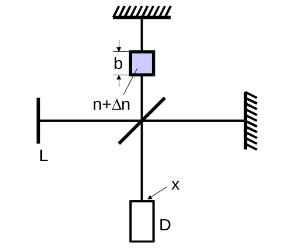
\includegraphics[scale = 0.5]{V401-Bild2.png}
  \caption{Schematischer Aufbau eines Michelson Interferometers zur Messung des Brechungsindizes \cite{Q1}.}
  \label{Abb:2}
\end{figure}

Das Medium der Dicke $d$ soll den Brechungsindex $ n + \Delta n$ besitzen und an allen anderen Stellen des Versuchs den Brechungsindex $n$. Wird $\Delta n$ nun langsam verändert,
entsteht an der Stelle $x$ ein oszillierendes Interferenzbild. Auch hier ist die Anzahl $z$ der Maxima für die Messung wichtig

\begin{equation}
  b \cdot \ \Delta n = z \cdot \frac{\lambda}{2}
\end{equation}

Um aus $\Delta n $ den Brechungsindex $n$ zu errechnen wird folgende Formel verwendet

\begin{equation}
  n(p_0,T_0) = 1 + \Delta n \frac{T \cdot p_0}{T_0 \cdot (p - p')}
\end{equation}

Wobei $T_0$ die Umgebungstemperatur und $p - p'$ die Druckdifferenz zum Umgebungsdruck darstellt.

\subsection{Versuchsaufbau}

Im Mittelpunkt des Versuchaufbaus steht das Michelson-Interferometer. Zur Verschiebung des Spiegels wird ein Synchronmotor angebracht, da die kontinuierliche Verschiebung in der Größenordnung
per Hand kaum möglich ist. Das eben benannte Medium wird hier als Messzelle dargestellt, durch die Vakuumpumpe ist es möglich, die Messzelle zumindest teilweise zu vakuumieren und
somit den Drruk $p$ und die Brechungsindex $n$ zu verändern. Außerdem wird direkt nach der Lichtquelle eine Zerstreuungslinse eingefügt, um ein konzentrisches Interferenzmuster darzustellen.

Um die Messung genauer zu machen, wird ein elektronisches Zählrohr für die Interferenzmaxima angebracht.
\begin{figure}
  \centering
  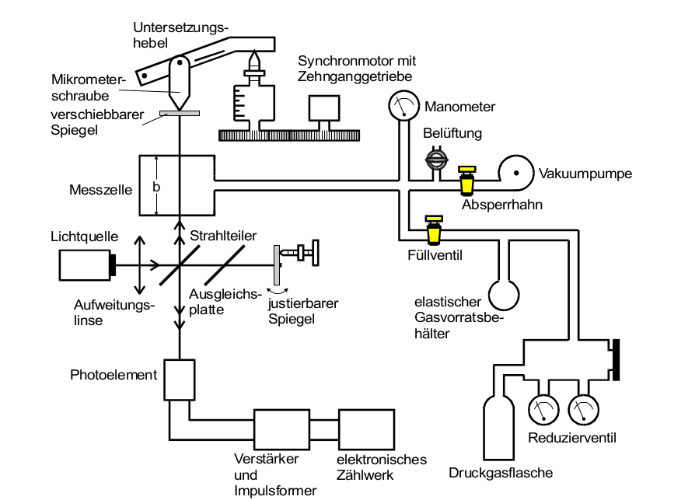
\includegraphics[scale = 0.5]{V401-Bild3.png}
  \caption{Versuchsaufbau \cite{Q1}.}
  \label{Abb:3}
\end{figure}

\section{Durchführung}
 Zu Beginn muss das Michelson-Interferometer genau justiert werden, dazu wird zunächst die Zerstreuungslinse herausgenommen und versucht die Maxima der beiden
 Strahlen auf dem Detektor überdeckend darzustellen, indem die Ausrichtung des Spiegels ohne Synchronmotor durch Drehen der Schrauben verstellt wird.
 Daraufhin wird die Zerstreuungslinse dem Versuchsaufbau hinzugefügt und der Detektor auf das innere Maximum des Interferenzbildes eingestellt.
 Zur Messung der Wellenlänge wird der Synchromotor und das Zählrohr eingeschaltet. Wenn das Zählrohr ca. 3000 Maxima gezählt hat, wird der Synchromotor ausgestellt
 und die Verschiebung $d$ des Spiegels abgelesen. Dieser Versuchsteil wird 10 mal durchgeführt.

 Zur Messung des Brechungsindizes wird die Messzelle so gut es geht vakuumiert und die Druckdifferenz zum Normaldruck abgelesen. Daraufhin wird das Zählrohr eingeschaltet und langsam
 die Luft wieder in die Messzelle gelassen. Wenn der Druck in der Messzelle wieder den Normaldruck erreicht hat, wird die Anzahl der Maxima am Zählrohr abgelesen.
 Der Versuchsteil wird 5 mal durchgeführt.

 \section{Auswertung}

\begin{table}
  \centering
  \label{tab1}
  \begin{tabular}{ c c c }
    \toprule
    {Anzahl der Maxima } & {$\Delta d $ / $\si{\milli \meter}$}  &  {$\lambda$ / $\nano \meter$} \\
    \midrule
  2999    &   4,94    &   656,65    \\
  3000    &   4,89    &   649,79    \\
  2999    &   4,93    &   655,32    \\
  3001    &   4,81    &   638,95    \\
  2999    &   4,86    &   646,02    \\
  3001    &   4,79    &   636,29    \\
  2998    &   4,86    &   646,24    \\
  3000    &   4,83    &   641,82    \\
  3000    &   5,02    &   667,07    \\
  2999    &   5,40    &   717,80    \\

   \bottomrule
 \end{tabular}
 \caption{Messwerte zur Bestimmung der Wellenlänge des Lasers.}
\end{table}

\noindent Der erste Teil des Versuchs besteht aus der Ermittlung der Wellenlänge des von dem Laser emittierten Lichts.
Hierfür wird Formel 3 verwendet. Die Ergebnisse sind zusammen mit den gemessenen Werten für
den Abstand von S1 zum Detektor in Tabelle \ref{tab1} zu finden. Hierbei ist darauf zu achten, dass Formel 3 um den Faktor
$\frac{1}{\symup{\ddot{U}}}$ erweitert werden muss. Ü ist die Hebelübersetzung, weshalb der abgelesene Wert für $d$
nicht der Tatsächlichen Verschiebung des Spiegels entspricht. Ü beträgt im Versuch 5,017.

\noindent Der Wert für $\lambda$ wird mit Hilfe folgener Formel gemittelt:

\begin{align*}
  \overline \lambda = \frac{1}{10} \sum_{i=1}^{10}{\lambda_i}
\end{align*}

\FloatBarrier
Anschließend wird der Fehler für die gemittelten Wellenlängen mit Hilfe folgender Formel berechnet:
\FloatBarrier

\begin{align*}
  \Delta \overline \lambda = \sqrt{\frac{1}{90} \sum_{i=1}^{10}{\left(\lambda_i - \overline \lambda \right)^2} }
\end{align*}
\FloatBarrier
Somit beträgt $\lambda$ \SI{655,60(749)}{\nano \meter}.



\subsection{Bestimmung des Brechungsindexes von Luft}
Folgende Werte sind vor der Berechnung des Brechungsindexes von Luft von Nöten:
\begin{align*}
  p_0 &= 1,0132 \symup{bar} \\
  b   &= 50 \milli \meter   \\
  T_0 &= 273,15 \kelvin     \\
  T   &= 293,15 \kelvin     \\
\end{align*}
\FloatBarrier
Hierbei beschreibt $p_0$ den Normaldruck, $b$ die Breite der Messzelle,$T_0$ die Normaltemperatur
und $T$ die Umgebungstemperatur. Diese wurde nicht explizit gemessen, jedoch betrug die Außentemperatur
am Tag des Versuchs $20 \si{\degree \celsius}$ und ein Fenster stand leicht geöffnet.
Mit Hilfe von Formel (2), in die Formel (3) nach der Umstellung nach $\Delta n$ eingesetzt wird,
werden dann die Brechungsindizes $n$ für jeden Messwert berechnet.

\FloatBarrier
\begin{align*}
  n(p_0,T_0) = 1 + \frac{z \lambda}{2b}\frac{T}{T_0}\frac{p_0}{\Delta p}
\end{align*}
\FloatBarrier
\begin{table}
  \centering
  \begin{tabular}{ c c c }
    \toprule
    {Anzahl der Maxima } & {$\Delta p $ / $\si{\bar}$} & {$n$}    \\
    \midrule
19    &   0,2332     &      1.000581 \pm  0.000007    \\
19    &   0,1732     &      1.000782 \pm  0.000009    \\
21    &   0,1731     &      1.000865 \pm  0.000010    \\
20    &   0,1532     &      1.000931 \pm  0.000011    \\
19    &   0,1732     &      1.000782 \pm  0.000009    \\

   \bottomrule
 \end{tabular}
 \caption{Messwerte zur Bestimmung des Brechungsindexes von Luft.}
 \label{tab2}
\end{table}

\noindent Die Ergebnisse befinden sich mit den
Messwerten in Tabelle \ref{tab2}. Da sich in der Berechnung des Brechungsindexes eine vorher gemittelte und
somit fehlerbehaftete Größe $\lambda$ befindet, muss hier die Gauß´sche Fehlerfortplanzung beachtet werden.
Der Fehler berechnet sich mittels folgender Formel:

\begin{align*}
  \Delta n = \sqrt{\left(\frac{z}{2b}\frac{T}{T_0}\frac{p_o}{\Delta p}\right)^2 (\Delta \lambda)^2}
\end{align*}

\FloatBarrier
Der gemittelte Wert für den Brechungsindex für Luft beträgt 1,000788 $\pm$ 0,000058.

\section{Diskussion}
Es ist zu erkennen, dass die Fehler bei beiden Messungen verhältnismäßig klein sind.
Dies lässt vermuten, dass die Messungen sehr präzise durchgeführt wurden.
Im Vergleich mit dem Literaturwert für den Brechungsindex von Luft 1,000272 \cite{Q2}
ist zu erkennen, dass sich der im Experiment ermittelte Wert von diesem erst in der vierten
Nachkommastelle unterscheidet. Dieser Unterschied ist zum Einen dadruch zu erklären, dass
der Versuchsaufbau extrem empfindlich ist und auch nur kleinste, ungewollte Berührungen des
Experimentiertisches das Messsystem bereits irritieren können. Zum Anderen ist der angegeben
Literaturwert der für den Brechungsindex von Luft bei Normaltemperatur. Im Versuch herrschten
jedoch Temperaturen über eben dieser. Auch wurde in den Berechnungen davon ausgegangen, dass
im Versuchsraum ein Normaldruck von 1,0132 bar herrschte, was mit Sicherheit auch nicht der
Realität entsprach. Allerdings lassen die geringen Fehler bei den durchgeführten Messungen
darauf schließen, dass keine systematischen Fehler in der Durchführung gemacht wurden.

\nocite{*}
\printbibliography
